\chapter{Logical Network Design}

\begin{figure}[ht]
    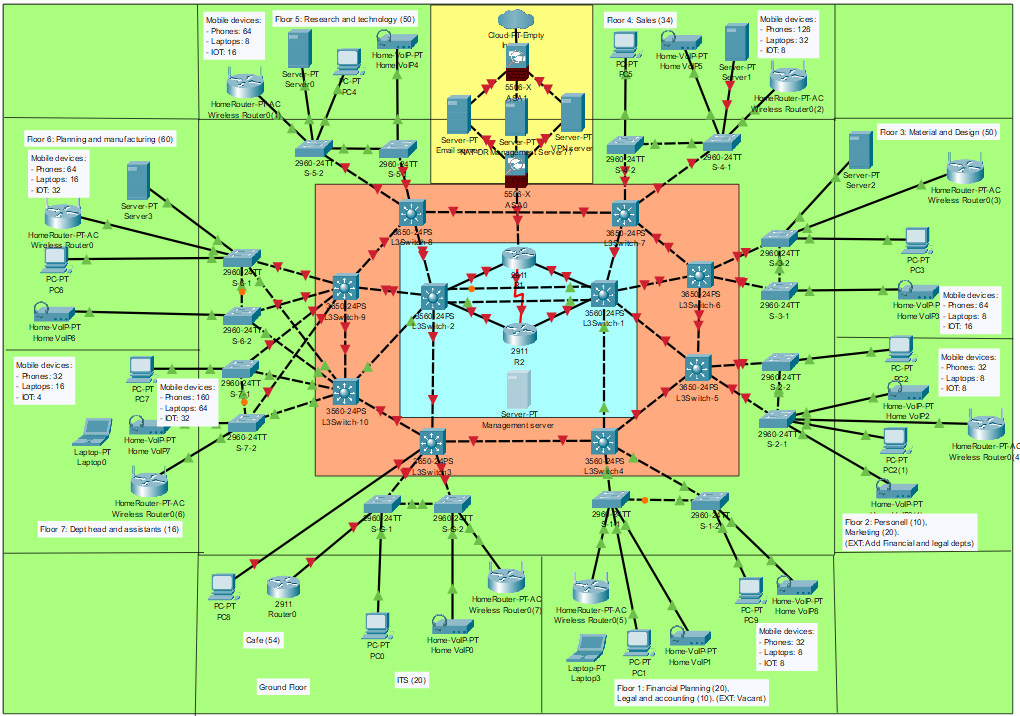
\includegraphics[width=15cm]{Figures/Network_Diagram.png}
    \caption{A Network Design produced in PacketTracer.}
    \label{fig:Network_Diagram}
\end{figure}

\section{Justifications}

The network diagram presented is a logical representation of the network being proposed. It is based on the assumptions of implementing the devices discussed earlier, as well as being secure and accessible for those who require it. See appendix section \ref{appendix:layered-model} for a guide to understanding the format.

\subsection{Server connections}
\begin{itemize}
    \item Management server: This server will be established as a core device that will provide a platform for managing the entire network, this device is only accessible from within the network itself and is provided access control mechanisms via R2.
    \item Email and VPN servers: Located within the DMZ, these servers are highly secured due to their increased risk of being attacked by entities attempting to contact them. They provide services to those working away from the office and help to manage the communication in and out of the network.
    \item Department servers: The departments that have dedicated servers are connected to the same switches to make sure they are secure and accessible
\end{itemize}
\subsection{Topology}
This design incorporates a hybrid mix of topologies to achieve the aim of being robust and tolerant to different types of operational problems. The mesh/ring structure of the core and distribution layers allows alternative paths and load balancing between the backbone devices of the network. The fully meshed connections between distribution and core layer switches gives a similar function, however with more redundancies.
\subsection{External facing router}
R1 is the router that is closest to the internet, it is behind the firewalls and connected to all components of the network via multiple links. It is heavily secured and monitored.
\subsection{Wireless access points}
Each department has their own WAP and block of IP addresses in order to divide the network for security purposes. 
\subsection{Private addressing scheme and implementation}
To provide the most addresses for the network we are using NAT/PAT, this private addressing allows us to be wasteful, and we have addressed the network accordingly. Each subnet has 254 addresses which is more than enough to consider expansion.